% This tells the program how to initially format my document.
\documentclass[dvipsnames]{article}

% List of packages to be included for the use of special commands and symbols.
\usepackage{amsmath,amssymb,amsthm}
\usepackage{mathtools}
\usepackage{mathrsfs}
\usepackage[letterpaper,margin=1in]{geometry}
\usepackage{enumitem}
%% remove ligatures (e.g. ``ff") to allow text copying from PDF
\usepackage{microtype}
\DisableLigatures{encoding = *, family = * }
\usepackage{fancyhdr}
\usepackage[T1]{fontenc}
\usepackage{lmodern}
\usepackage[USenglish]{babel}

\usepackage{tikz}
\usepackage{float}
\usepackage{listings}
\usepackage{xcolor}
\usepackage{multicol}
\usepackage{subcaption}

\newcommand{\ints}{\mathbb{Z}}

\definecolor{lispgreen}{RGB}{154, 228, 151}
\definecolor{lightgray}{gray}{0.97}
\definecolor{violet}{rgb}{0.8, 0, 0.7}

\lstdefinestyle{cpp}{
    language=C++,
	basicstyle=\fontsize{9}{11}\ttfamily,
	keywordstyle=\color{blue}\ttfamily,
	stringstyle=\color{red}\ttfamily,
	commentstyle=\color{OliveGreen}\ttfamily,
	morecomment=[l][\color{magenta}]{\#},
	tabsize=2,
    showstringspaces=false,
    backgroundcolor=\color{lightgray},
    numbers=left,
    stepnumber=5,
    numberstyle=\tiny
}
\lstdefinestyle{out}{
    basicstyle=\fontsize{9}{11}\ttfamily,
    tabsize=4,
    backgroundcolor=\color{lightgray},
    morecomment=[l][\color{OliveGreen}]{\#},
    numbers=none
}

\setlength{\parindent}{0cm}

\pagestyle{fancy}
\rhead{\large Alexander Novotny}
\lhead{\large CS 485 PA2}
\setlength{\headheight}{14pt}

\title{CS 485 Programming Assignment 2}
\date{April 7, 2019}
\author{Alexander Novotny}

\begin{document}
\pagenumbering{roman}

\maketitle

\section*{Problem 1 - Toon Shading}
\subsection*{Approach}
\begin{enumerate}
	\item Break the image into three separate intensity sub-images based on color space.
	\item Discretize each sub-image intensity into $l$ buckets, where $l = 2,4,8,16$.
	\item Loop through each pixel of each sub-image, putting them into a bucket by changing the intensity value to the bucket number. Also keep track of the average intensity in each bucket.
	\item Go back through the image, replacing each bucket value with the average intensity for that bucket.
\end{enumerate}

\subsection*{Color Space}
The BGR color space was used, as this is the default color space used by OpenCV. Since each member of the color space was compressed equally, there wasn't any particular need to use another color space.

\subsection*{Equations used}
To quantize the space, we have $b : \ints^2 \to \{0,1,2,\dots,l-1\}$,
\begin{equation}
	b(x,y) = \left\lfloor\frac{l*I(x,y)}{I_{max} + 1}\right\rfloor,
\end{equation}
where $b(x,y)$ is the bucket the pixel at $(x,y)$ belongs to, $l$ is the quantization-level, $I(x,y)$ is the intensity of the pixel at $(x,y)$ and $I_{max}$ is the maximum intensity the pixel can have (with the assumption that the minimum is always 0). For all $B,G,R$ we have $I_{max} = 255$. Note that for $I(x,y) = I_{max}$ then $b(x,y) = l - 1$.\\

As well, I kept track of an average intensity value $\mu_n$ for each pixel in each bucket,
\begin{equation}
	\mu_n = \frac{I_1 + I_2 + \dots + I_n}{n},
\end{equation}
where $I_i$ is the intensity of a pixel in the bucket and there are $n$ such pixels in the bucket. Since at any point in time we don't know how many more pixels will be in this bucket, I wanted to be able to calculate and update this number without storing each previous intensity value. A naive way to do this might be to keep track of $n$ and $S_n = I_1 + I_2 + \dots + I_n = S_{n-1} + I_n$, however this can easily overflow. So instead I considered a moving average
\begin{align}
	\mu_{n+1} &= \frac{S_{n+1}}{n + 1} \nonumber\\
	          &= \frac{S_n + I_{n+1}}{n + 1} \nonumber\\
	          &= \frac{S_n}{n+1} + \frac{I_{n+1}}{n+1} \nonumber\\
	          &= \frac{S_n}{n}\left(\frac{n}{n+1}\right) + \frac{I_{n+1}}{n+1} \nonumber\\
	          &= \mu_n\left(\frac{n}{n+1}\right) + \frac{I_{n+1}}{n+1},
\end{align}
so I only have to keep track of the current moving average $\mu_n$ and the number of pixels stored in each bin $n$.

\subsection*{Results}
\begin{figure}[H]
	\centering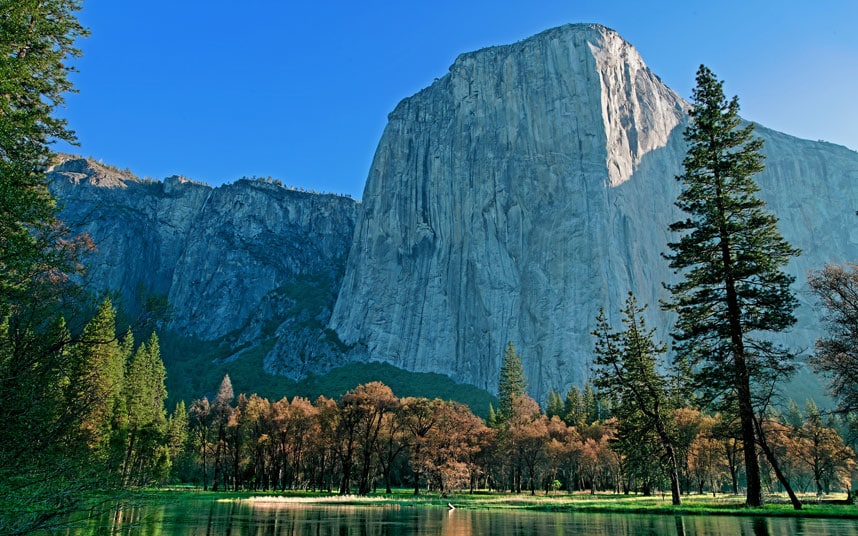
\includegraphics[width=.5\linewidth]{Images/P-1/ElCapitan.jpg}
	\caption{Original ElCapitan.jpg}

	\begin{subfigure}{.33\linewidth}
		\centering\includegraphics[width=\linewidth]{Out/P-1/ElCapitan-toon-2.jpg}
		\caption{Toon shading with $l = 2$}
	\end{subfigure}
	\begin{subfigure}{.33\linewidth}
		\centering\includegraphics[width=\linewidth]{Out/P-1/ElCapitan-toon-4.jpg}
		\caption{Toon shading with $l = 4$}
	\end{subfigure}
	\begin{subfigure}{.33\linewidth}
		\centering\includegraphics[width=\linewidth]{Out/P-1/ElCapitan-toon-8.jpg}
		\caption{Toon shading with $l = 8$}
	\end{subfigure}
	\begin{subfigure}{.33\linewidth}
		\centering\includegraphics[width=\linewidth]{Out/P-1/ElCapitan-toon-16.jpg}
		\caption{Toon shading with $l = 16$}
	\end{subfigure}
\end{figure}

\begin{figure}[H]
	\centering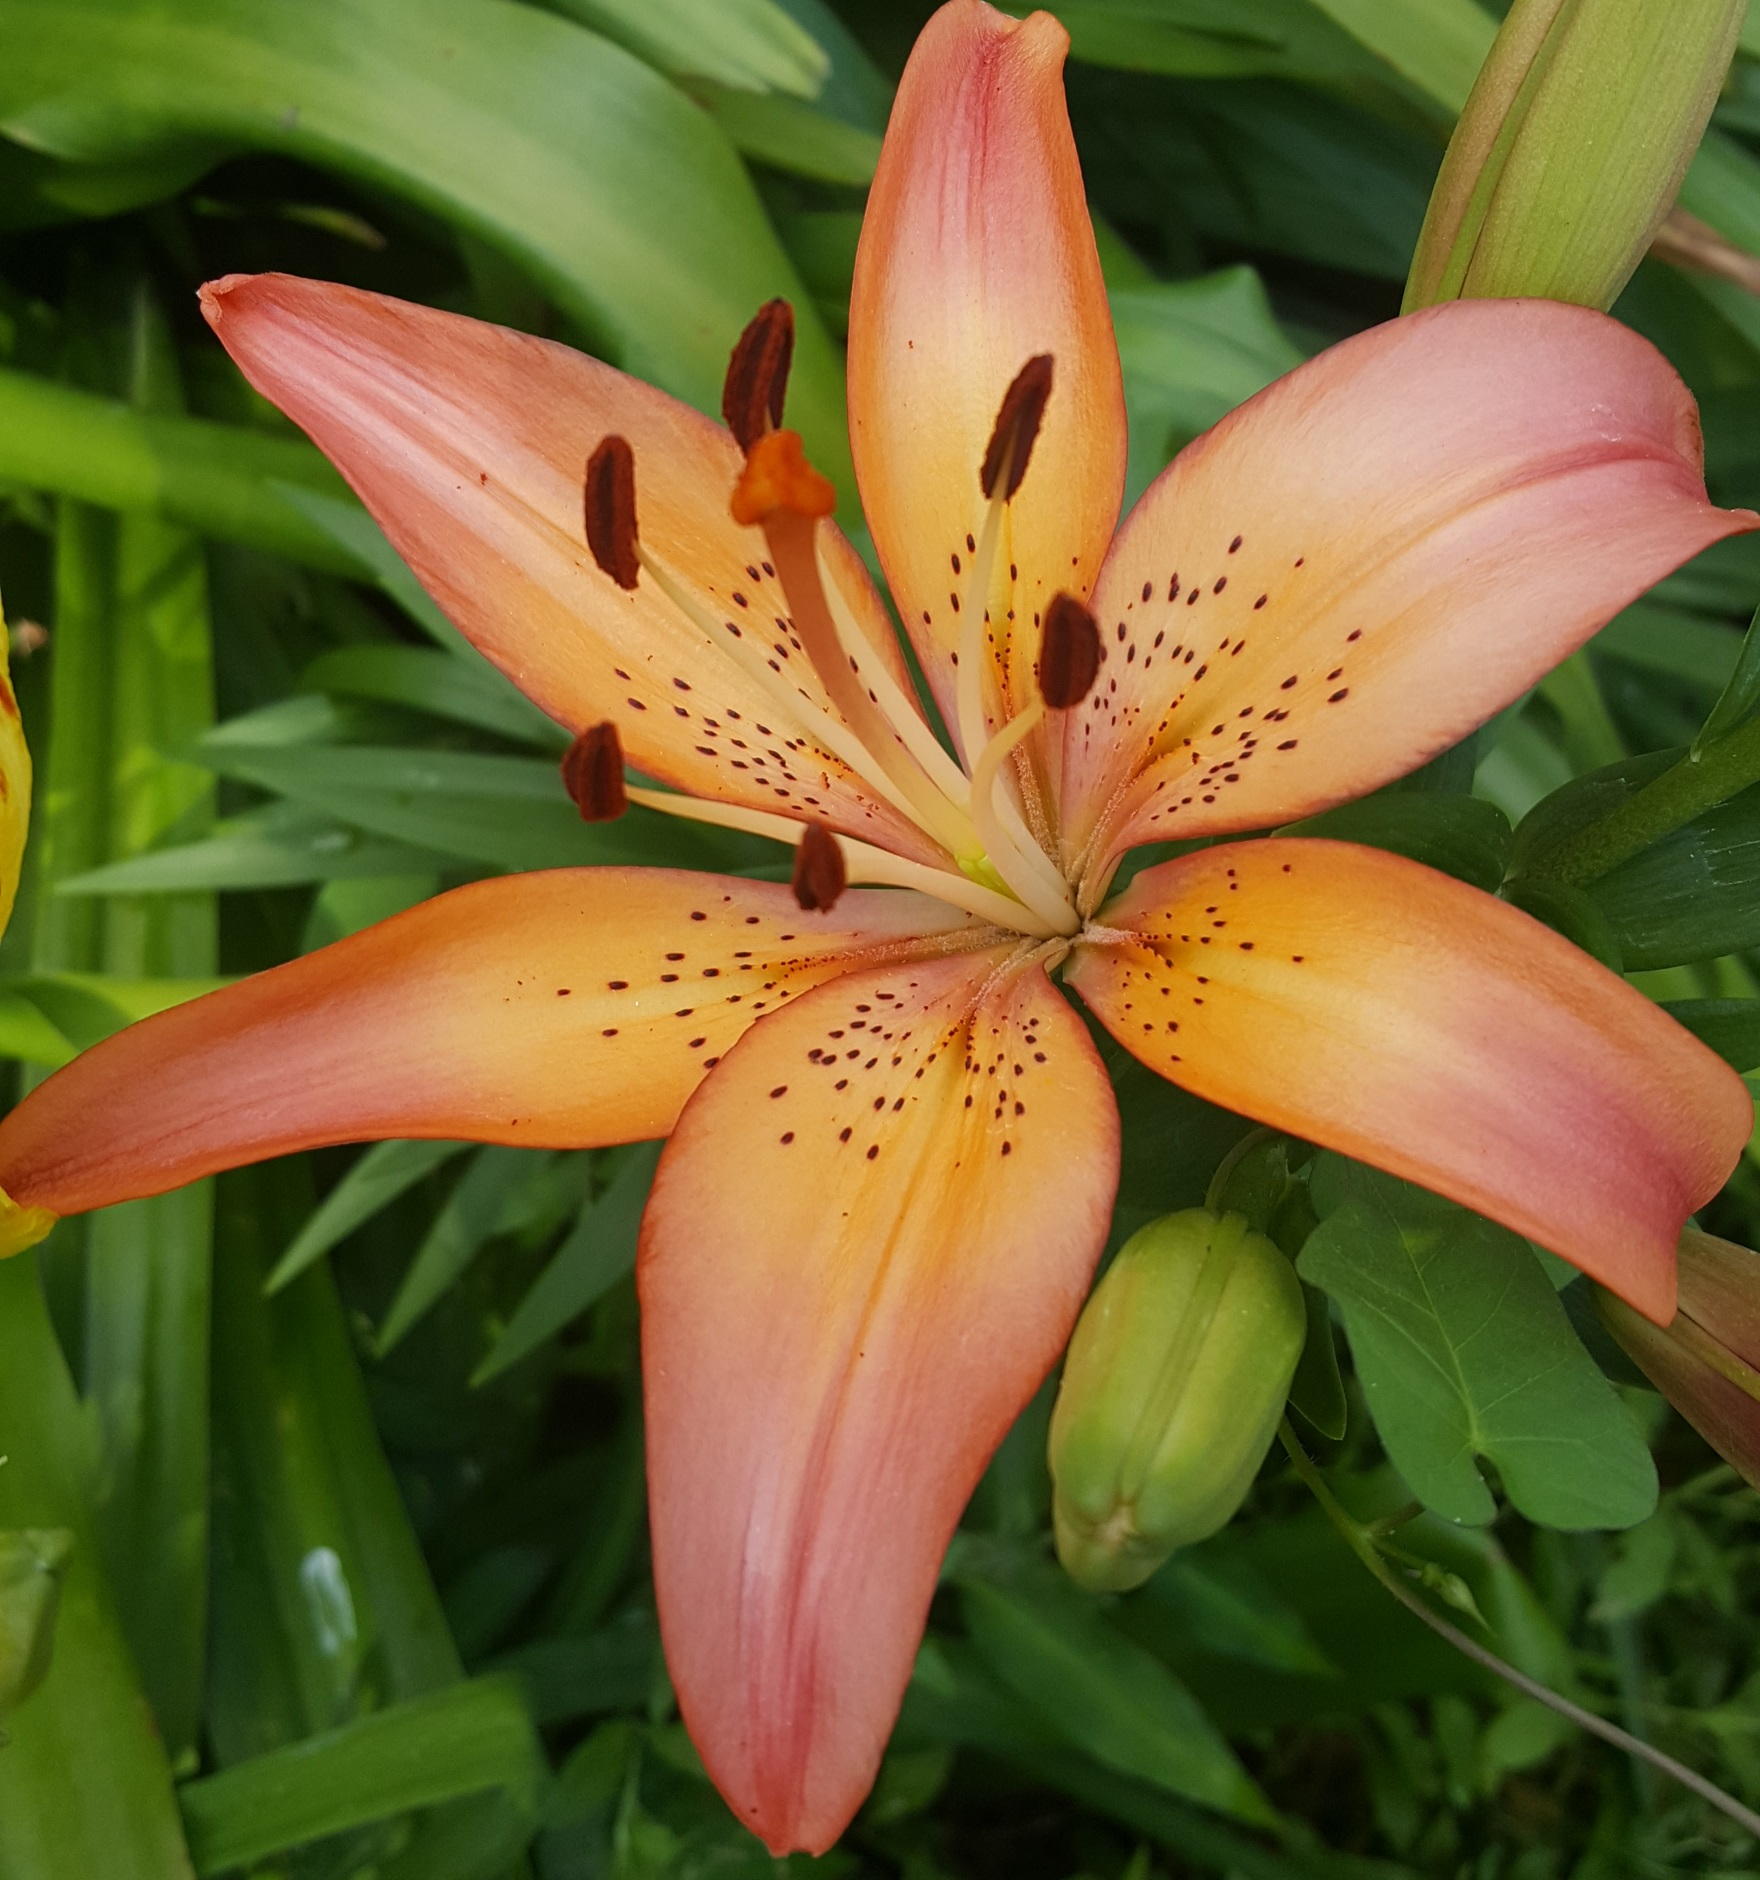
\includegraphics[width=.5\linewidth]{Images/P-1/Lilly.jpg}
	\caption{Original Lilly.jpg}

	\begin{subfigure}{.33\linewidth}
		\centering\includegraphics[width=\linewidth]{Out/P-1/Lilly-toon-2.jpg}
		\caption{Toon shading with $l = 2$}
	\end{subfigure}
	\begin{subfigure}{.33\linewidth}
		\centering\includegraphics[width=\linewidth]{Out/P-1/Lilly-toon-4.jpg}
		\caption{Toon shading with $l = 4$}
	\end{subfigure}
	\begin{subfigure}{.33\linewidth}
		\centering\includegraphics[width=\linewidth]{Out/P-1/Lilly-toon-8.jpg}
		\caption{Toon shading with $l = 8$}
	\end{subfigure}
	\begin{subfigure}{.33\linewidth}
		\centering\includegraphics[width=\linewidth]{Out/P-1/Lilly-toon-16.jpg}
		\caption{Toon shading with $l = 16$}
	\end{subfigure}
\end{figure}

\begin{figure}[H]
	\centering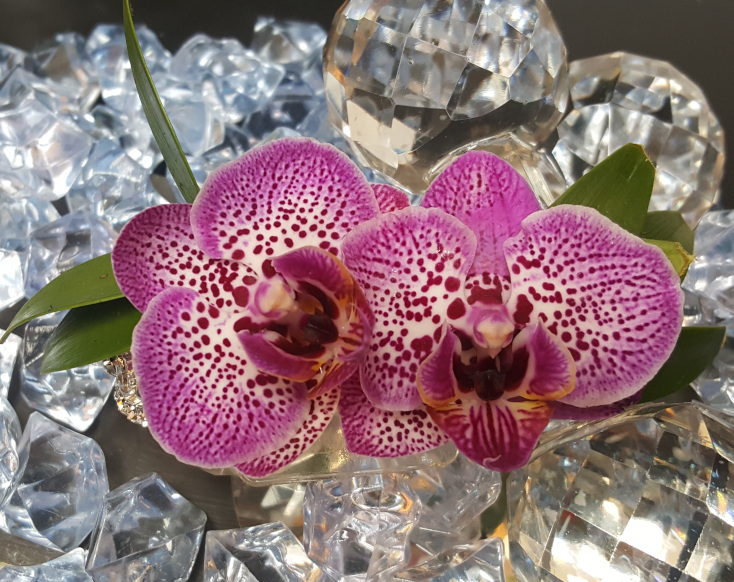
\includegraphics[width=.5\linewidth]{Images/P-1/Orchids.jpg}
	\caption{Original Orchids.jpg}

	\begin{subfigure}{.33\linewidth}
		\centering\includegraphics[width=\linewidth]{Out/P-1/Orchids-toon-2.jpg}
		\caption{Toon shading with $l = 2$}
	\end{subfigure}
	\begin{subfigure}{.33\linewidth}
		\centering\includegraphics[width=\linewidth]{Out/P-1/Orchids-toon-4.jpg}
		\caption{Toon shading with $l = 4$}
	\end{subfigure}
	\begin{subfigure}{.33\linewidth}
		\centering\includegraphics[width=\linewidth]{Out/P-1/Orchids-toon-8.jpg}
		\caption{Toon shading with $l = 8$}
	\end{subfigure}
	\begin{subfigure}{.33\linewidth}
		\centering\includegraphics[width=\linewidth]{Out/P-1/Orchids-toon-16.jpg}
		\caption{Toon shading with $l = 16$}
	\end{subfigure}
\end{figure}

\begin{figure}[H]
	\centering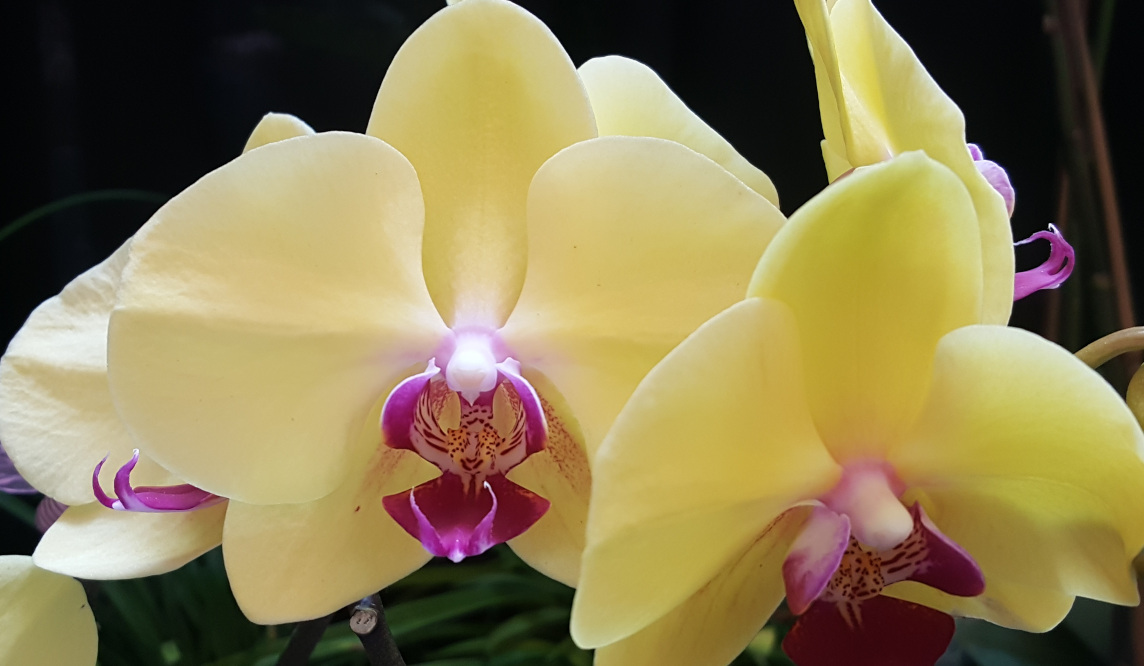
\includegraphics[width=.5\linewidth]{Images/P-1/OrchidsY.jpg}
	\caption{Original OrchidsY.jpg}

	\begin{subfigure}{.33\linewidth}
		\centering\includegraphics[width=\linewidth]{Out/P-1/OrchidsY-toon-2.jpg}
		\caption{Toon shading with $l = 2$}
	\end{subfigure}
	\begin{subfigure}{.33\linewidth}
		\centering\includegraphics[width=\linewidth]{Out/P-1/OrchidsY-toon-4.jpg}
		\caption{Toon shading with $l = 4$}
	\end{subfigure}
	\begin{subfigure}{.33\linewidth}
		\centering\includegraphics[width=\linewidth]{Out/P-1/OrchidsY-toon-8.jpg}
		\caption{Toon shading with $l = 8$}
	\end{subfigure}
	\begin{subfigure}{.33\linewidth}
		\centering\includegraphics[width=\linewidth]{Out/P-1/OrchidsY-toon-16.jpg}
		\caption{Toon shading with $l = 16$}
	\end{subfigure}
\end{figure}

\begin{figure}[H]
	\centering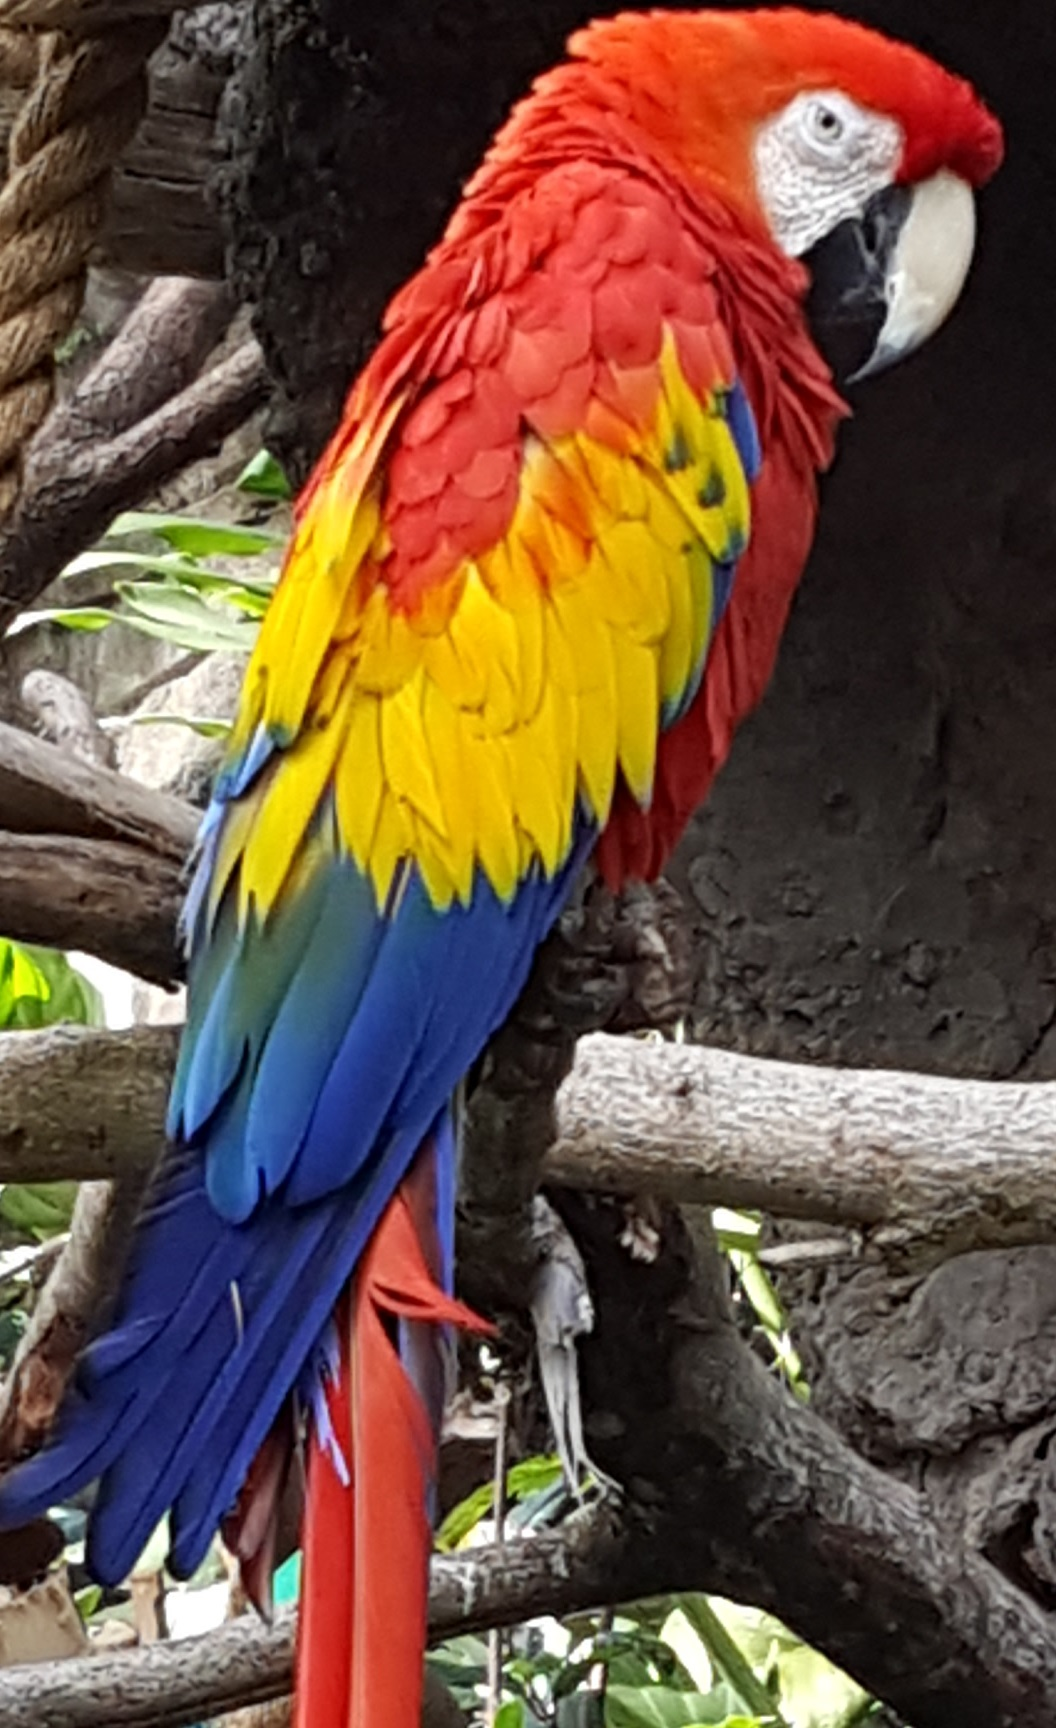
\includegraphics[height=.5\linewidth]{Images/P-1/Parrot.jpg}
	\caption{Original Parrot.jpg}

	\begin{subfigure}{.33\linewidth}
		\centering\includegraphics[height=\linewidth]{Out/P-1/Parrot-toon-2.jpg}
		\caption{Toon shading with $l = 2$}
	\end{subfigure}
	\begin{subfigure}{.33\linewidth}
		\centering\includegraphics[height=\linewidth]{Out/P-1/Parrot-toon-4.jpg}
		\caption{Toon shading with $l = 4$}
	\end{subfigure}
	\begin{subfigure}{.33\linewidth}
		\centering\includegraphics[height=\linewidth]{Out/P-1/Parrot-toon-8.jpg}
		\caption{Toon shading with $l = 8$}
	\end{subfigure}
	\begin{subfigure}{.33\linewidth}
		\centering\includegraphics[height=\linewidth]{Out/P-1/Parrot-toon-16.jpg}
		\caption{Toon shading with $l = 16$}
	\end{subfigure}
\end{figure}

\section*{Problem 1 - Color Compression}
\subsection*{Approach}
\begin{enumerate}
	\item Break the image into three separate intensity sub-images based on color space (HSV).
	\item Discretize the saturation sub-image.
	\item Loop through each pixel of the sub-image, finding the bucket each pixel belongs to and replacing the intensity with the minimum intensity for that bucket.
\end{enumerate}

An average approach was considered, similar to toon shading, however this did not produce images similar to the ones in the project description.

\subsection*{Color Space}
The color space which was used was HSV, as the type of color is encoded entirely in Hue, so we can compress saturation without affecting the type of color present in the pixel.

\subsection*{Results}
\begin{figure}[H]
	\centering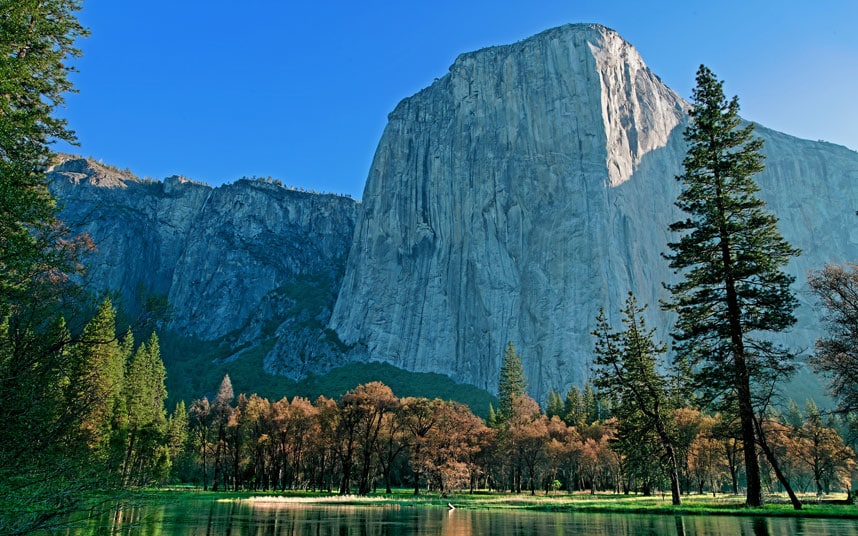
\includegraphics[width=.5\linewidth]{Images/P-1/ElCapitan.jpg}
	\caption{Original ElCapitan.jpg}

	\begin{subfigure}{.33\linewidth}
		\centering\includegraphics[width=\linewidth]{Out/P-1/ElCapitan-comp-2.jpg}
		\caption{Color compressed with $l = 2$}
	\end{subfigure}
	\begin{subfigure}{.33\linewidth}
		\centering\includegraphics[width=\linewidth]{Out/P-1/ElCapitan-comp-4.jpg}
		\caption{Color compressed with $l = 4$}
	\end{subfigure}
	\begin{subfigure}{.33\linewidth}
		\centering\includegraphics[width=\linewidth]{Out/P-1/ElCapitan-comp-8.jpg}
		\caption{Color compressed with $l = 8$}
	\end{subfigure}
	\begin{subfigure}{.33\linewidth}
		\centering\includegraphics[width=\linewidth]{Out/P-1/ElCapitan-comp-16.jpg}
		\caption{Color compressed with $l = 16$}
	\end{subfigure}
\end{figure}

\begin{figure}[H]
	\centering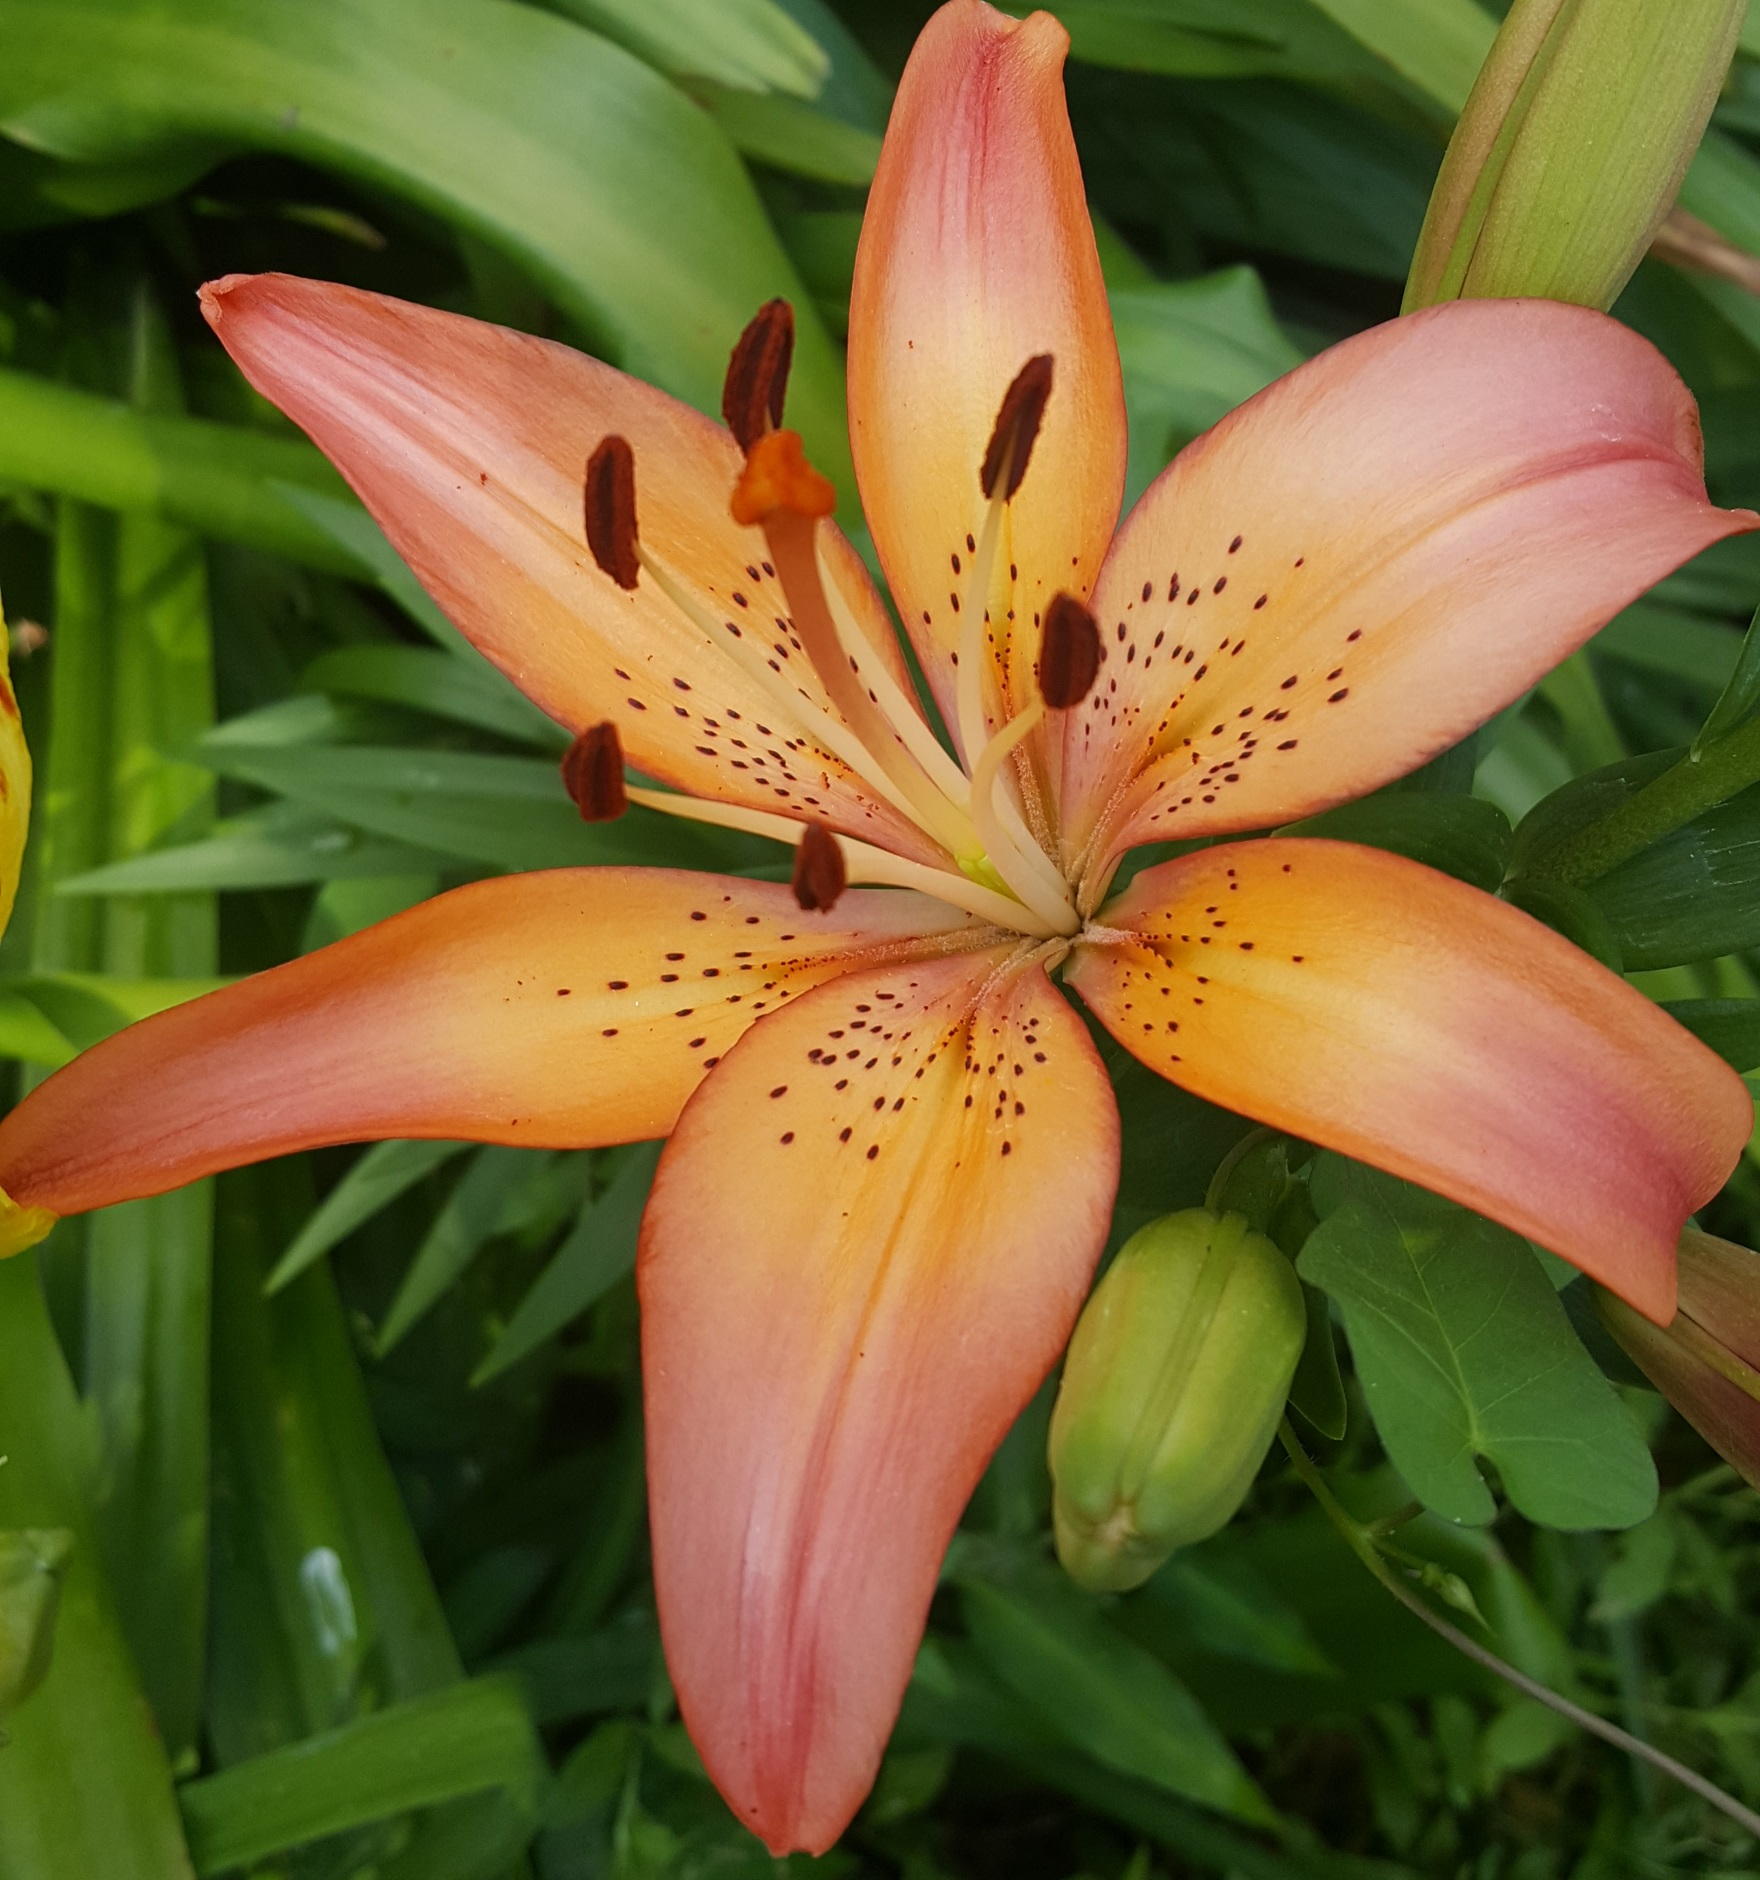
\includegraphics[width=.5\linewidth]{Images/P-1/Lilly.jpg}
	\caption{Original Lilly.jpg}

	\begin{subfigure}{.33\linewidth}
		\centering\includegraphics[width=\linewidth]{Out/P-1/Lilly-comp-2.jpg}
		\caption{Color compressed with $l = 2$}
	\end{subfigure}
	\begin{subfigure}{.33\linewidth}
		\centering\includegraphics[width=\linewidth]{Out/P-1/Lilly-comp-4.jpg}
		\caption{Color compressed with $l = 4$}
	\end{subfigure}
	\begin{subfigure}{.33\linewidth}
		\centering\includegraphics[width=\linewidth]{Out/P-1/Lilly-comp-8.jpg}
		\caption{Color compressed with $l = 8$}
	\end{subfigure}
	\begin{subfigure}{.33\linewidth}
		\centering\includegraphics[width=\linewidth]{Out/P-1/Lilly-comp-16.jpg}
		\caption{Color compressed with $l = 16$}
	\end{subfigure}
\end{figure}

\begin{figure}[H]
	\centering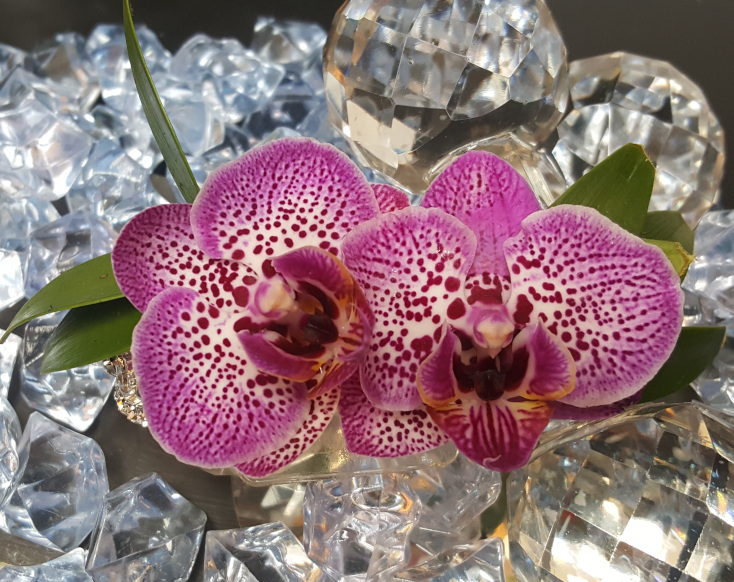
\includegraphics[width=.5\linewidth]{Images/P-1/Orchids.jpg}
	\caption{Original Orchids.jpg}

	\begin{subfigure}{.33\linewidth}
		\centering\includegraphics[width=\linewidth]{Out/P-1/Orchids-comp-2.jpg}
		\caption{Color compressed with $l = 2$}
	\end{subfigure}
	\begin{subfigure}{.33\linewidth}
		\centering\includegraphics[width=\linewidth]{Out/P-1/Orchids-comp-4.jpg}
		\caption{Color compressed with $l = 4$}
	\end{subfigure}
	\begin{subfigure}{.33\linewidth}
		\centering\includegraphics[width=\linewidth]{Out/P-1/Orchids-comp-8.jpg}
		\caption{Color compressed with $l = 8$}
	\end{subfigure}
	\begin{subfigure}{.33\linewidth}
		\centering\includegraphics[width=\linewidth]{Out/P-1/Orchids-comp-16.jpg}
		\caption{Color compressed with $l = 16$}
	\end{subfigure}
\end{figure}

\begin{figure}[H]
	\centering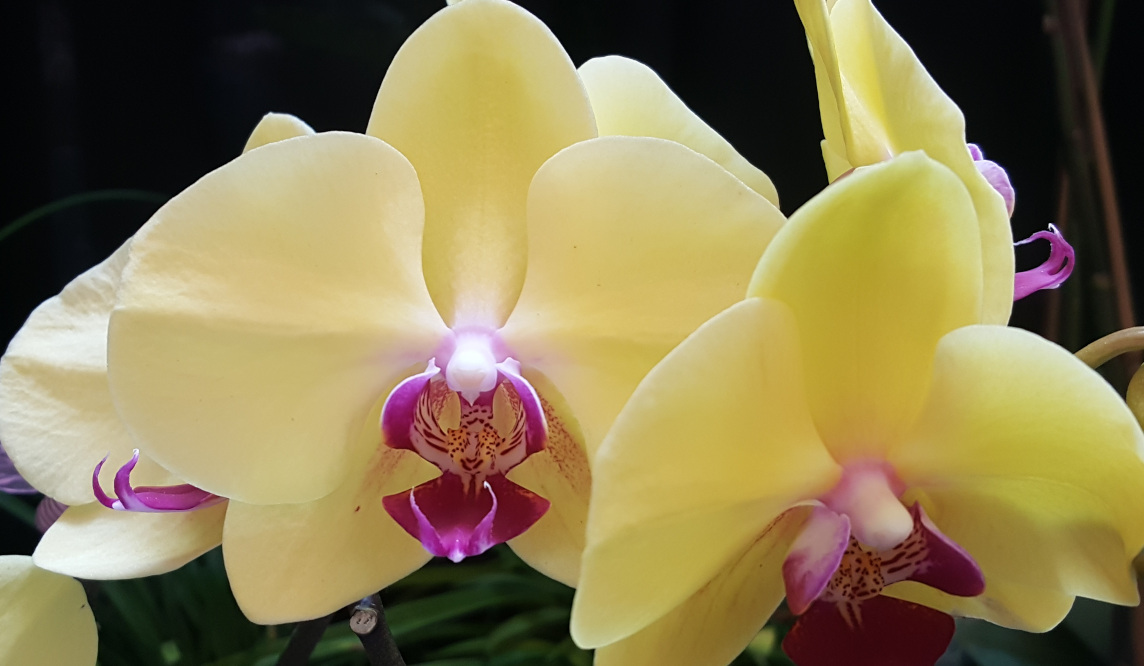
\includegraphics[width=.5\linewidth]{Images/P-1/OrchidsY.jpg}
	\caption{Original OrchidsY.jpg}

	\begin{subfigure}{.33\linewidth}
		\centering\includegraphics[width=\linewidth]{Out/P-1/OrchidsY-comp-2.jpg}
		\caption{Color compressed with $l = 2$}
	\end{subfigure}
	\begin{subfigure}{.33\linewidth}
		\centering\includegraphics[width=\linewidth]{Out/P-1/OrchidsY-comp-4.jpg}
		\caption{Color compressed with $l = 4$}
	\end{subfigure}
	\begin{subfigure}{.33\linewidth}
		\centering\includegraphics[width=\linewidth]{Out/P-1/OrchidsY-comp-8.jpg}
		\caption{Color compressed with $l = 8$}
	\end{subfigure}
	\begin{subfigure}{.33\linewidth}
		\centering\includegraphics[width=\linewidth]{Out/P-1/OrchidsY-comp-16.jpg}
		\caption{Color compressed with $l = 16$}
	\end{subfigure}
\end{figure}

\begin{figure}[H]
	\centering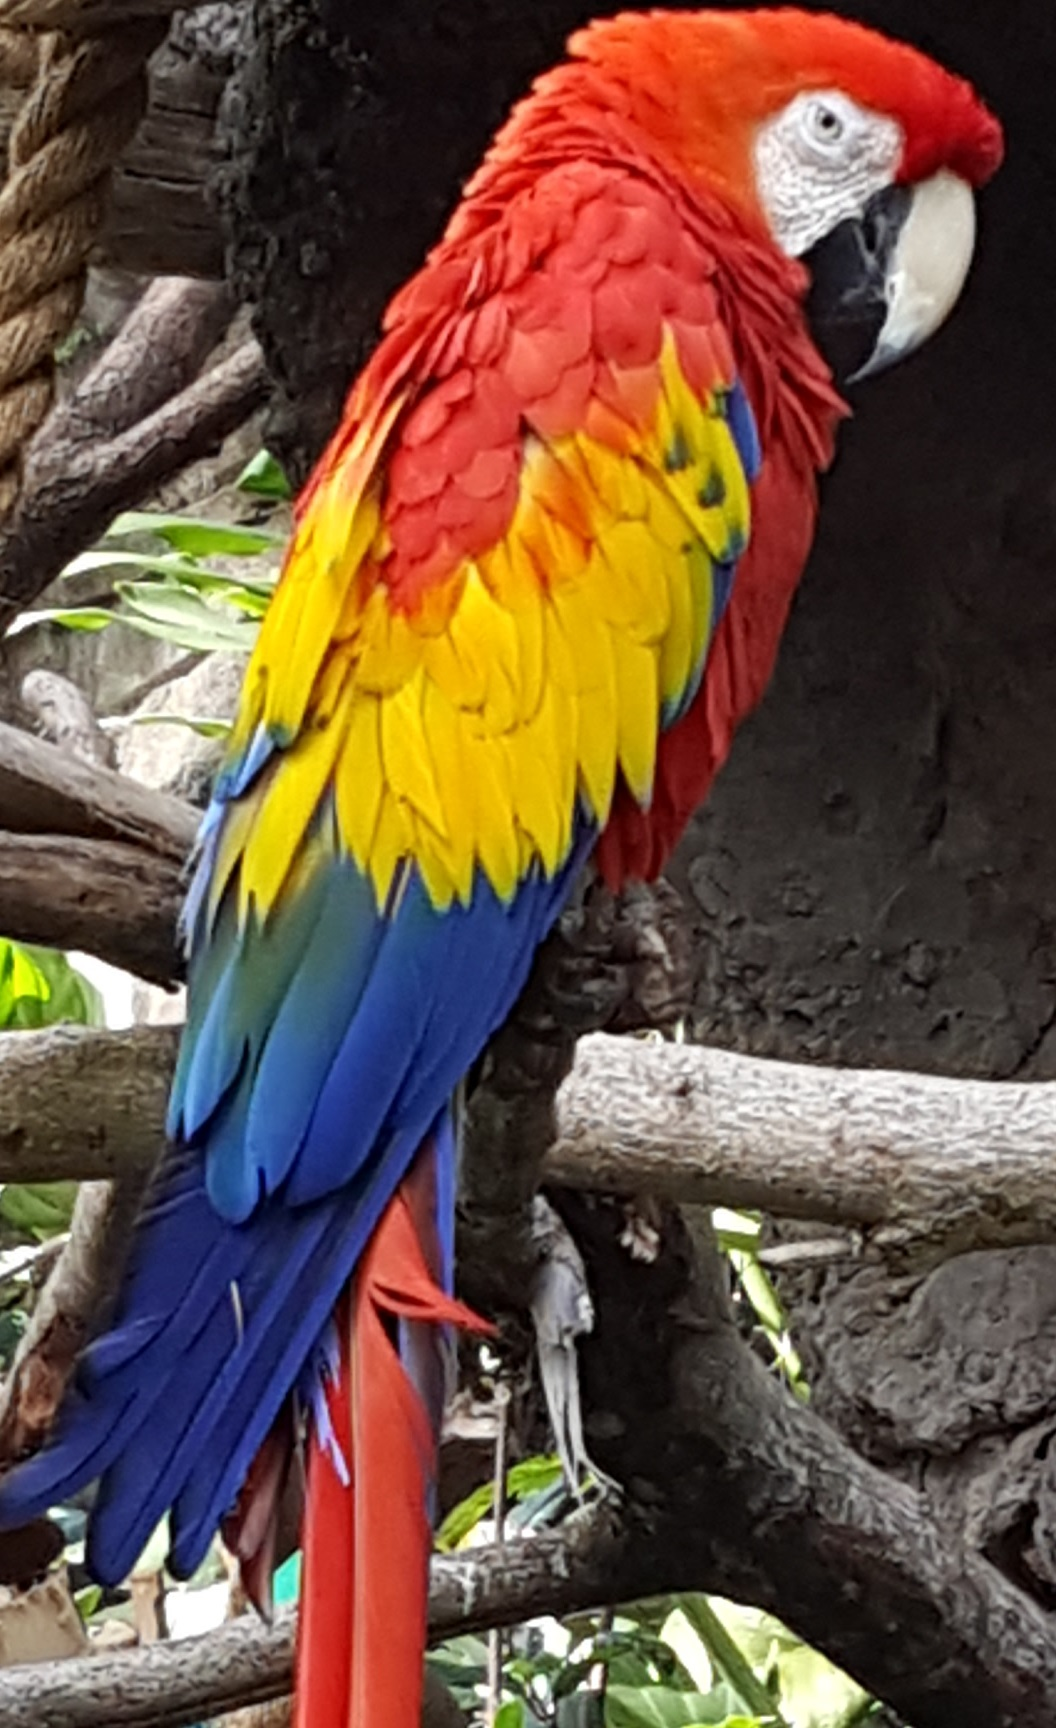
\includegraphics[height=.5\linewidth]{Images/P-1/Parrot.jpg}
	\caption{Original Parrot.jpg}

	\begin{subfigure}{.33\linewidth}
		\centering\includegraphics[height=\linewidth]{Out/P-1/Parrot-comp-2.jpg}
		\caption{Color compressed with $l = 2$}
	\end{subfigure}
	\begin{subfigure}{.33\linewidth}
		\centering\includegraphics[height=\linewidth]{Out/P-1/Parrot-comp-4.jpg}
		\caption{Color compressed with $l = 4$}
	\end{subfigure}
	\begin{subfigure}{.33\linewidth}
		\centering\includegraphics[height=\linewidth]{Out/P-1/Parrot-comp-8.jpg}
		\caption{Color compressed with $l = 8$}
	\end{subfigure}
	\begin{subfigure}{.33\linewidth}
		\centering\includegraphics[height=\linewidth]{Out/P-1/Parrot-comp-16.jpg}
		\caption{Color compressed with $l = 16$}
	\end{subfigure}
\end{figure}

\section*{Problem 2 - Hough Transform Circle Detection}
\subsection*{Approach}

\begin{enumerate}
	\item Discretize possible radius values into buckets
	\item Find all trees of each radius bucket, starting from the smallest
	\item If a tree already exists in one of these locations, there can't be another. So throw out the duplicate
\end{enumerate}

\subsection*{Results}
\begin{figure}[H]
	\centering\includegraphics[width=.75\linewidth]{Images/P-2/LiDAR01-circled.png}
	\caption{LIDAR with trees circled}
\end{figure}

The run time for the program was .468716 seconds. The detection results were a bit unsatisfactory, but a large majority of the objects detected were actual trees and a large majority of the trees were detected.

\end{document}